\documentclass[a4paper, 12pt, oneside]{extbook}
\usepackage[T1]{fontenc}
\usepackage[utf8]{inputenc}
\usepackage{geometry}
\usepackage{courier}
\usepackage{listings}
\lstset{language=bash}

\usepackage[bookmarks]{hyperref}
\newgeometry{
left=   1.5 in,
bottom= 1.5 in,
right=  1 in,
top=    1 in
}

\usepackage{fancyhdr}

% Grafica
\usepackage{graphicx,pstricks}
\usepackage{graphics}
\graphicspath{{img/}}

% Package usati per il frontespizio
\usepackage{tikz}
\usepackage{pgf-pie}
\usepackage{pgfplots}
\pgfplotsset{width=7cm,compat=1.8}
\usetikzlibrary{patterns}


\setlength\headheight{44.2pt}
%Page Style
\usepackage{setspace}
%\setstretch{2.5} 
%\doublespace

%\cfoot{\thepage}
\lhead[]{}
\rhead[]{\leftmark}

\pagestyle{fancy}{
\lhead{
\includegraphics[scale=0.3]{img/logo/hlogo.png}}
\rhead{\footnotesize{Elaborato Network Security}}
}

%Other
\usepackage{comment}
\usepackage{amsmath}

%Testo riempitivo
\usepackage{lipsum}




\begin{document}

%\maketitle
\begin{titlepage}
\thispagestyle{empty}
\raggedright % Allinea a sinistra

\begin{tikzpicture}
\node[anchor=south west] at (4,0) {
\includegraphics[scale=0.75]{img/logo/logo_copertina_1}};
\node[anchor=south west] at (0,1.5) {
\includegraphics{img/logo/logo_copertina_2}};
\node[anchor=south west] at (0,0.5) {\textsf{Scuola Politecnica e delle Scienze di Base}};
\node[anchor=south west] at (0,0) {\textsf{Corso di Laurea Magistrale in Ingegneria Informatica}};
\end{tikzpicture}

\vfill

{\textbf{\textit{\LARGE Elaborato di Network Security}}}
\\[1cm]
{\large Anno Accademico 2022/2023}

\vfill


\begin{table}[h]
{\raggedright}

\textbf{Christian Marescalco}

\textbf{matr. M63001367}

\textbf{Antonio Avolio}

\textbf{matr. M63001352}
\end{table}

\end{titlepage}
\frontmatter

{\setstretch{1.5}
\tableofcontents
}

\mainmatter
\chapter{Footprinting}
The footprinting phase involves gathering information in the network regarding the target,in our case the organization and its members.
\newline In this scenario, the attacker already knows information regarding the company and has managed to connect to the target local network.
\newline Through the ifconfig tool he discovers the subnets to which he is connected: Employee Network, Company Network.
\newline ifconfig screen
\newline Using the nmap tool, the attacker discovers the topology of the various subnets within the organization, identifying the target ip's of the web server and employee computers
\begin{center}
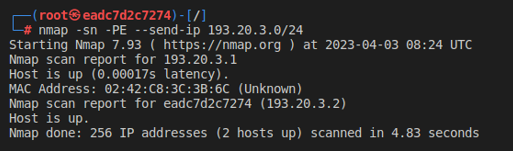
\includegraphics[scale=1]{../Image/footprinting_company_network.png}
\end{center}
\begin{lstlisting}
  nmap -sn -PE --send-ip 193.20.3.0/24
\end{lstlisting}
From the top scan of the IP range 193.20.3.0/24 Bob found out one host up at 193.20.3.1 and his MAC Address.
\begin{center}
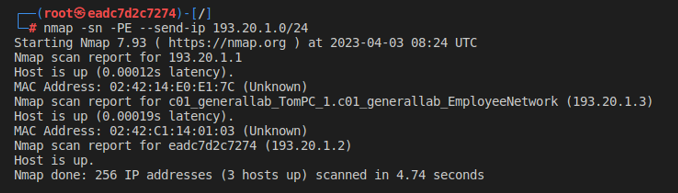
\includegraphics[scale=0.76]{../Image/footprinting_employee_network.png}
\end{center}
\newpage
\chapter{Scanning}
Nmap (Network Mapper) is a versatile and powerful tool with a range of options and features. Here are some of the main options:
\begin{itemize}
  \item Host Discovery: This option is used to discover hosts on a network. Nmap can identify active hosts, as well as those that are currently offline.
  \item Port Scanning: Port scanning is one of the most popular features of Nmap. It can be used to identify open ports on a target system, and even detect hidden ports and services.
  \item Service and Version Detection: This option is used to identify the services and versions of software running on the target system. This information can be useful in identifying vulnerabilities and weaknesses.
  \item Operating System Detection: Nmap can also be used to identify the operating system running on the target system. This information can be helpful in identifying potential attack vectors.
  \item Scripting Engine: Nmap has a powerful scripting engine that allows users to write and execute custom scripts. This feature can be used to automate tasks, customize scans, and extend the functionality of Nmap.
  \item Output Formats: Nmap can generate output in various formats, including XML, HTML, and plain text. This feature can be helpful in generating reports, analyzing results, and sharing information with others.
\end{itemize} 
These are just a few of the main options available in Nmap. Other features include traceroute, firewall detection, and performance tuning options. Nmap is a highly flexible tool that can be customized to suit the needs of the user.
It has a number of flags or options that can be used to customize and fine-tune its scanning behavior.
\newline Here are some commonly used flag options:
\begin{itemize}
  \item \textbf{-sS}: This flag specifies the type of scan to be performed, in this case a SYN scan.
  \item \textbf{-sT}: This flag specifies a TCP connect scan, where Nmap attempts to establish a full TCP connection with the target ports.
  \item \textbf{-sU}: This flag specifies a UDP scan, where Nmap sends UDP packets to the target ports and listens for responses.
  \item \textbf{-sC}: This flag specifies a scan usiong the default set of scripts. Some of the scripts in this category are considered intrusive.
  \item \textbf{-O}: This flag enables operating system detection, allowing Nmap to identify the operating system running on the target system.
  \item \textbf{-p}: This flag specifies the ports to be scanned, and can take a range of values or a comma-separated list of individual port numbers.
  \item \textbf{-oN}: This flag specifies the output format for Nmap results, in this case, plain text format.
  \item \textbf{-oN}: This option is used to specify the output format of the scan results. For example, the command "nmap -oN output.txt" will save the scan results to a file called "output.txt".
\end{itemize}
These are just a few examples of the flag options available in Nmap.
\end{document}